\chapter{Results}
Here we list several different kinds of results for the window search method and the gradient assisted window search method.  We present measures in the form of average number of word replacements per sample, time taken to converge, number of algorithm failures, as well as the transferability to different models with a similar architecture.  In each case, we discard samples which were incorrectly classified in the first place, and use a single layer recurrent neural network with a hidden layer of size 16 as the base model.  We measure the performace of each method over the same 500 randomly chosen samples.  

\section{White Box}
Here we assume that all details of the model are known including the exact weights.  We determine candidate word replacements based on inferring with those weights directly.  figures \ref{fig:succwindow} and \ref{fig:cumwindow} show the distribution of the number of words required to change a classification and the cumulative distribution respectively.
\begin{figure}
    \centering
    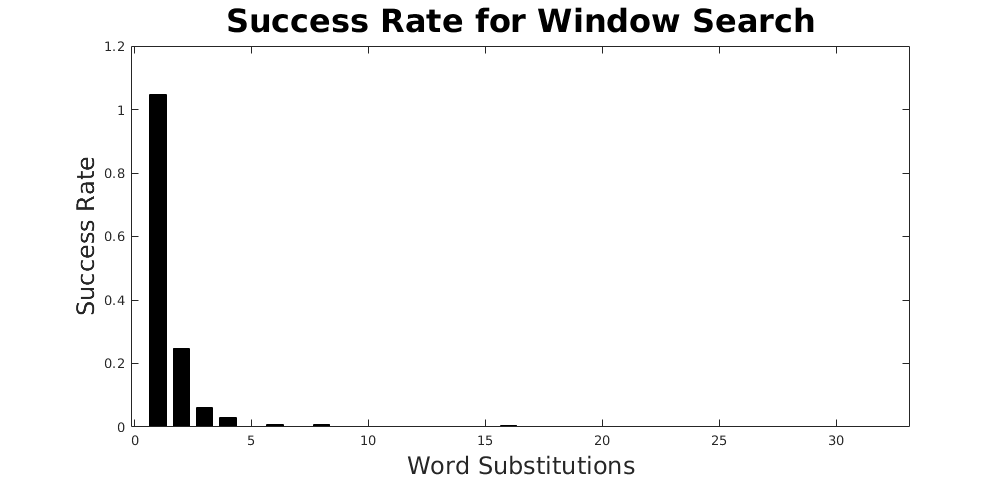
\includegraphics[width=\textwidth]{succwindow.png}
    \caption{Success rate for window search vs. number of word substitutions required.}
    \label{fig:succwindow}
\end{figure}
\begin{figure}
    \centering
    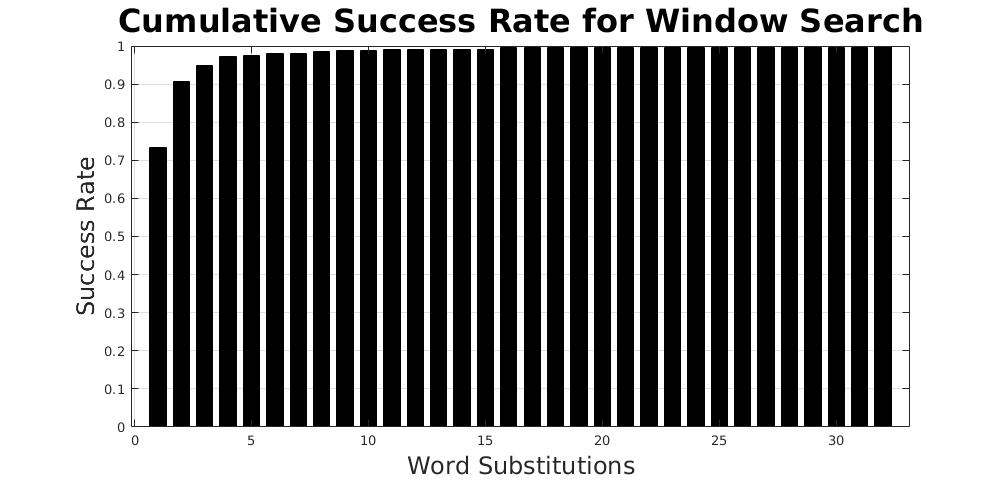
\includegraphics[width=\textwidth]{cumwindow.png}
    \caption{Cumulative success rate for window search vs. number of word substitutions required.}
    \label{fig:cumwindow}
\end{figure}

Gradient assisted window search achieved a mean of 2.25 words per misclassification, median of 2, and mode of 1.  Figure \ref{fig:succgaws} and \ref{fig:cumgaws} show the distribution of words required to change a classification and the cumulative distribution respectively.  Figure \ref{fig:timegaws} shows the distribution of time required to either achieve misclassification or recognize that the algorithm has failed to do so.
\begin{figure}
    \centering
    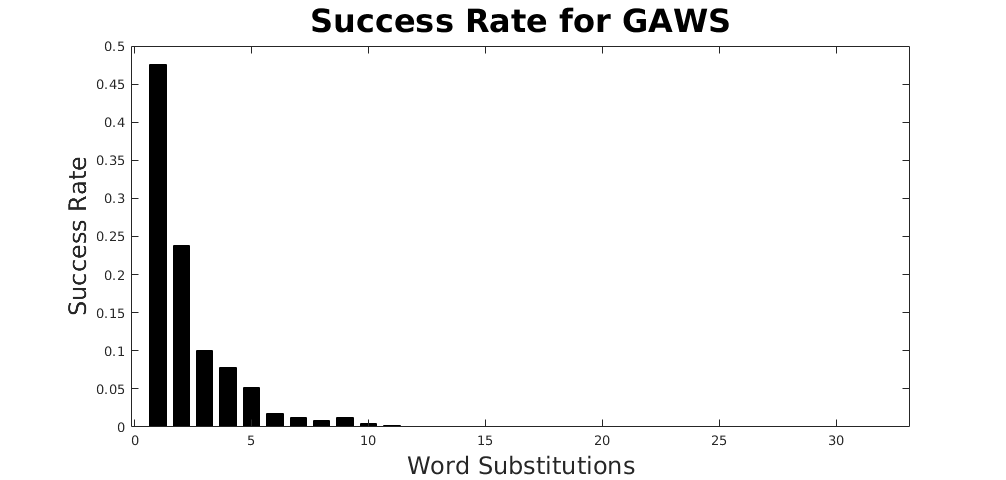
\includegraphics[width=\textwidth]{succgaws.png}
    \caption{Success rate for window search vs. number of word substitutions required.}
    \label{fig:succgaws}
\end{figure}
\begin{figure}
    \centering
    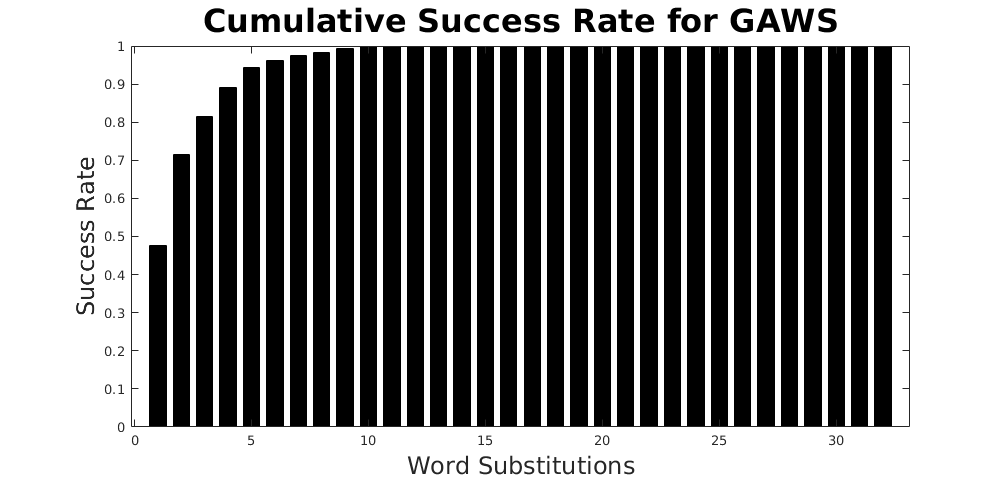
\includegraphics[width=\textwidth]{cumgaws.png}
    \caption{Cumulative success rate for window search vs. number of word substitutions required.}
    \label{fig:cumgaws}
\end{figure}
\begin{figure}
    \centering
    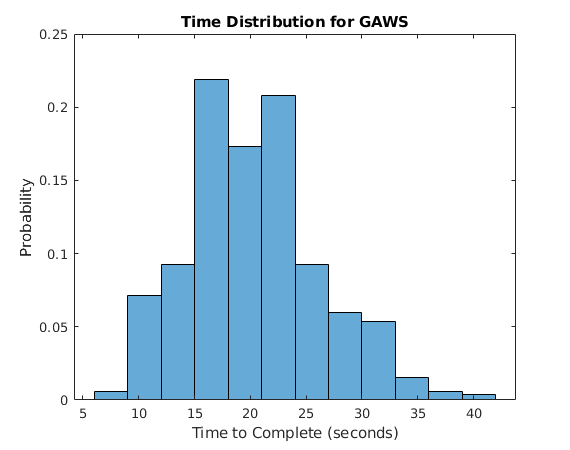
\includegraphics[width=\textwidth]{timegaws.png}
    \caption{Distribution of time required for the GAWS algorithm}
    \label{fig:timegaws}
\end{figure}

\section{Gray Box}
General structure of model known including hyperparameters
 algorithm run on stand-in model trained on same data, but not same model.
\section{Black Box}
Here we assume that no details of the model are known, in particular the hyperparameters are uknown.  In order to evaluate performace under this condition, we determine word substitutions using an RNN with a hidden layer of size 16 and attack an RNN with a hidden layer size of 8.  
